\documentclass[border=0.8ex,svgnames,tikz]{standalone}
\usepackage{amsmath,mathtools}
\usepackage{fontspec}
\setmainfont{Source Serif 4}
\setsansfont{Source Sans 3}
\setmonofont{Source Code Pro}
\usetikzlibrary{calc,positioning}
\begin{document}
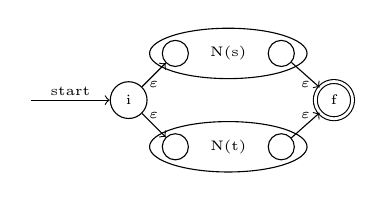
\begin{tikzpicture}
  \node[text width=-3em](Start){};
  \node[circle, draw=black, right= of Start](RI){\tiny i};
  \node[circle, draw=black, above right=1.21em of RI](SI){};
  \node[circle, draw=black, right= of SI](SF){};
  \node[circle, draw=black, below right=1.21em of RI](TI){};
  \node[circle, draw=black, right= of TI](TF){};
  \node[circle, double, double distance=1pt, draw=black, right=1.21em of $(SF)!0.5!(TF)$](RF){\tiny f};

  \path[->]
  (Start) edge node[above=-2pt]{\tiny start} (RI)
  (RI) edge node[above=-8pt]{\tiny $\varepsilon$} (SI)
  (SI) edge[draw=none] node{\tiny N(s)} (SF)
  (SF) edge node[above=-8pt]{\tiny $\varepsilon$} (RF)
  (RI) edge node[below=-8pt]{\tiny $\varepsilon$} (TI)
  (TI) edge[draw=none] node{\tiny N(t)} (TF)
  (TF) edge node[below=-8pt]{\tiny $\varepsilon$} (RF);

  \draw ($(SF)!0.5!(SI)$) ellipse (1 and 0.32);
  \draw ($(TF)!0.5!(TI)$) ellipse (1 and 0.32);
\end{tikzpicture}
\end{document}
